\documentclass{article}

\usepackage[T1]{fontenc}    %Schriftart des Dokumentes
\usepackage[ngerman]{babel} %Dokumentensprache, hier Deutsch
\usepackage{amsmath, amssymb, stmaryrd} %mathematische Schriftzeichen
\usepackage{graphicx} %Einfügen von Grafiken
\usepackage{wrapfig}
\usepackage{bm}

\setlength{\parindent}{0pt} %Einrückung von Absätzen auf null gesetzt
\setlength{\parskip}{10pt} %Abstand zischen Absätzen auf 10pt gesetzt

\title{Versuch 22: Bestimmung der Elementarladung nach Millikan}
\author{Matthias Kuntz}
\date{27.09.2023}

\begin{document}

\maketitle

%-------------------------EINLEITUNG-------------------------
\section{Einleitung}

In diesem Versuch wollen wir die Elementarladung $e$ mit einer Methode bestimmen, die erstmals 1913 von Robert A. Millikan veröffentlicht wurde und ihm später den Nobelpreis für Physik vermachte. Dazu beobachten wir Öltröpchen in einem Plattenkondensator, um deren Fallgeschwindigkeit bei ausgeschaltetem und deren Steiggeschwindigkeit bei angeschaltetem Kondensator zu bestimmen.  

\subsection{Physikalische Grundlagen}

Millikans Versuch basiert darauf, dass auf ein Tröpfchen im Kondensator verschiedene Kräfte wirken. Diese sind

\begin{equation}
    \begin{split}
        \text{die Gewichtskraft}& \ \ \ F_G = \frac{4}{3}\pi r^3 \rho_{"ol}g, \\
        \text{die Auftriebskraft}& \ \ \ F_A = \frac{4}{3}\pi r^3 \rho_{luft}g, \\
        \text{die Stokessche Reibung}& \ \ \ F_R = 6\pi r\eta v \ \ \ \text{und} \\
        \text{die elektrische Kraft}& \ \ \ F_E = q\frac{U}{d}. \\
    \end{split}
    \label{eq:kräfte}
\end{equation}

Hierbei sind $r$ der Radius des Tröpfchens, $\rho$ die Dichte von Öl beziehungsweise Luft, $g$ die Fallbeschleunigung, $\eta$ die Viskosität der Luft, $v$ die Geschwindigkeit des Tröpchens, $q$ dessen Ladung, $U$ die Spannung auf dem Kondenstaor und $d$ der Abstand von dessen Platten. Die elektrische Kraft wirkt natürlich nur bei eingeschaltetem Kondensator. 

Lässt man zunächst den Kondensator ausgeschaltet, so kann man mit der Fallgeschwindigkeit eines Tröpfchens $v_f$ aus der Summe der drei wirkenden Kräfte den Radius $r$ bestimmen:

\begin{equation}
    r = \sqrt{\frac{9\eta}{2\rho g}v_f}
    \label{eq:r}
\end{equation}

Hierbei bezeichnet $\rho$ die Differenz der Dichte von Öl und Luft: $\rho = \rho_{"ol} - \rho_{luft}$.

Schaltet man den kondensator ein und betrachtet die Steiggeschwindigkeit eines Tröpfschens $v_s$ kann man die Ladung $q$ bestimmen:

\begin{equation}
    q = (v_f + v_s) \sqrt{\frac{9v_f \eta^3}{2 \rho g}} \frac{6 \pi d}{U}
    \label{eq:q}
\end{equation}

Bei der Versuchsauswertung muss beachtet werden, dass die Viskosität $\eta$ bei kleinen Öltröpfchen, wie die von uns betrachteten, nicht konstant ist und durch einen radiusabhängigen Korrekturfaktor $f(r)$ korrigiert werden muss:

\begin{equation}
    \eta(r) = \eta_0 f(r) = \frac{\eta_0}{1+\frac{b}{rp}}
    \label{eq:eta}
\end{equation}

Dabei sind $\eta_0$ der Grenzwert der Viskosität für sehr große Tröpfchen, $b$ eine empirische Konstante und $p$ der Luftdruck. 

\subsection{Versuchsaufbau}

Eine genaue Skizze des Versuchsaufbaus ist auf der nächsten Seite im Messprotokoll dargestellt.

Der Aufbau von Millikan besteht aus einem Plattenkondensator, in den mit einem Ölzersteuber kleine Tröpfen eingelassen werden können. Eine Lampe beleuchtet dabei den Zwischenraum, welcher von einer Kamera mit Mikroskop gefilmt wird und das Bild vergrößert sowie mit einer Skala versehen auf einem Bildschirm darstellt. Ein Steuergerät dient zum Ein- und Ausschalten des Kondensators sowie zum Starten und Stoppen zweier Stoppuhren, eine für den eingeschalteten und eine für den ausgeschalteten Zustand. Während des Versuchs tragen wir die Messwerte in eine gestellte Excel-Tabelle ein, welche bereits so konfiguriert wurde, dass automatisch alle nötigen Zwischenwerte und schlussendlich die Ladungen aller Tröpfchen berechnet werden. 

%---------------VERSUCHSPROTOKOLL MIT MESSDATEN---------------
\newpage

\section{Versuchsprotokoll mit Messdaten}

\includegraphics[width=\textwidth]{graphics/mess1.jpg}
\newpage
\includegraphics[width=\textwidth]{graphics/mess2.jpg}
\newpage
\includegraphics[width=\textwidth]{graphics/mess3.jpg}
\newpage

\addtocounter{table}{2}

%-------------------------AUSWERTUNG-------------------------
\section{Auswertung}

In dieser Evaluation werden alle Fehler, sofern keine spezifische Angabe gemacht wird, mithilfe der Gauss'schen Fehlerfortpflanzung berechnet. Dies bedeutet, dass ein Wert $F$, der mit der Formel $f(a_1, ..., a_n)$ berechnet wird, den Fehler $\Delta F$ gegeben über folgende Formel hat:

\begin{equation}
    \Delta F = \sqrt{\sum_n \left( \frac{\partial f}{\partial a_n} \cdot \Delta a_n \right)^2}.
\end{equation}

\subsection{Untersuchung eines einzelnen Tröpfchens}

Wir beginnen, indem wir ein Tröpfchen aus Tabelle 2 auswählen, wir entscheiden uns für den Eintrag 42, und manuell Steig- und Fallgeschwindigkeit $v_s$ \& $v_f$ sowie den Radius $r_0$, $f(r_0)$ und die Ladung $q$ berechnen. Der Einfachheit halber werden erstmal keine Fehler berechnet. Eintrag 42 hat folgende Ausgangswerte: eine Strecke von 21 Skalenteilen, $t_s = 18,380$s und $t_f = 35,860$s. Wir beginnen mit den Geschwindigkeiten. Zunächst bestimmen wir die Strecke mit den Angaben der Skalenlänge:

\begin{equation}
    \begin{split}
        1 \ \text{Skt} &= (5,00 \pm 0,13) \cdot 10^{-5} \text{m} \\ \\
        s = 21 \ \text{Skt} &= (1,050 \pm 0,027) \cdot 10^{-3} \text{m}
    \end{split}
    \label{r:s}
\end{equation}

Nun können wir damit die Geschwindigkeiten bestimmen:

\begin{equation}
    \begin{split}
        v &= \frac{s}{t} \\ \\%, \ \ \ \ \Delta v = v \sqrt{\left( \frac{\Delta s}{s} \right)^2 + \left( \frac{\Delta t}{t} \right)^2} \\ \\
        v_s &= 0,0571 \cdot 10^{-3} \frac{\text{m}}{\text{s}} \\
        v_f &= 0,0293 \cdot 10^{-3} \frac{\text{m}}{\text{s}} \\
    \end{split}
    \label{r:v}
\end{equation}

Nun nutzen wir Gleichung \ref{eq:r} um den Radius $r_0$ zu bestimmen. Wir nutzen $\eta_0 = 1,81 \cdot 10^{-5} \frac{\text{Ns}}{\text{m}^2}$ und $\rho = \rho_{"o} - \rho_L$, mit $\rho_{"o} = 871 \frac{\text{kg}}{\text{m}^3}$ und $\rho_{L} = 1,29 \frac{\text{kg}}{\text{m}^3}$:

\begin{equation}
    \begin{split}
        r_0 &= \sqrt{\frac{9 \eta_0}{2 \rho g}v_f} \\ \\%, \ \ & \ \ \Delta r_0 = \sqrt{\frac{9 \eta_0}{8 \rho g}} \cdot \frac{\Delta v_f}{\sqrt{v_f}} \\ \\
        r_0 &= 0,5289 \cdot 10^{-6} \text{m}
    \end{split}
\end{equation}

Damit bestimmen wir $f(r_0)$ nach Gleichung \ref{eq:eta}. Wir verwenden $b=7,78 \cdot 10^{-3}\text{Pa m}$ und den gemessen Wert $p_L = (1008,7 \pm 0,1)$hPa:

\begin{equation}
    \begin{split}
        f(r_0) &= \frac{1}{1+\frac{b}{r_0p_L}} \\ \\%, \ \ \ \Delta f(r_0) &= \frac{b}{\left( b+p_Lr_0 \right)^2} \sqrt{(p_L \cdot \Delta r_0)^2 + (r_0 \cdot \Delta p_L)^2} \\ \\
        f(r_0) &= 0,8726
    \end{split}
\end{equation}

Zuletzt können wir die Ladung $q$ mit Gleichung \ref{eq:q} bestimmen, wobei gilt $U = (500 \pm 1)$V, $d = 6,00 \pm 0,05$mm und $\eta = \eta_0 * f(r)$:

\begin{equation}
\begin{split}
    q &= (v_f + v_s) \sqrt{\frac{9v_f \eta^3}{2 \rho g}} \frac{6 \pi d}{U} \\ \\
    %\Delta q &= \\ \\
    q &= 1,5251 \cdot 10^{-19} \text{C}    
\end{split}
\end{equation}

Somit lässt sich feststellen, dass alle händisch berechneten Werte praktisch 1:1 mit den Werten der Tabelle übereinstimmen, nur der bestimmte Wert für $q$ weicht ab der dritten Nachkommastelle um 1 ab, was wohl auf Rundungsfehler zurückzuführen ist.

\newpage

\subsection{Histogramm der gemessenen Ladungen}

\begin{figure} [!h]
    \centering
    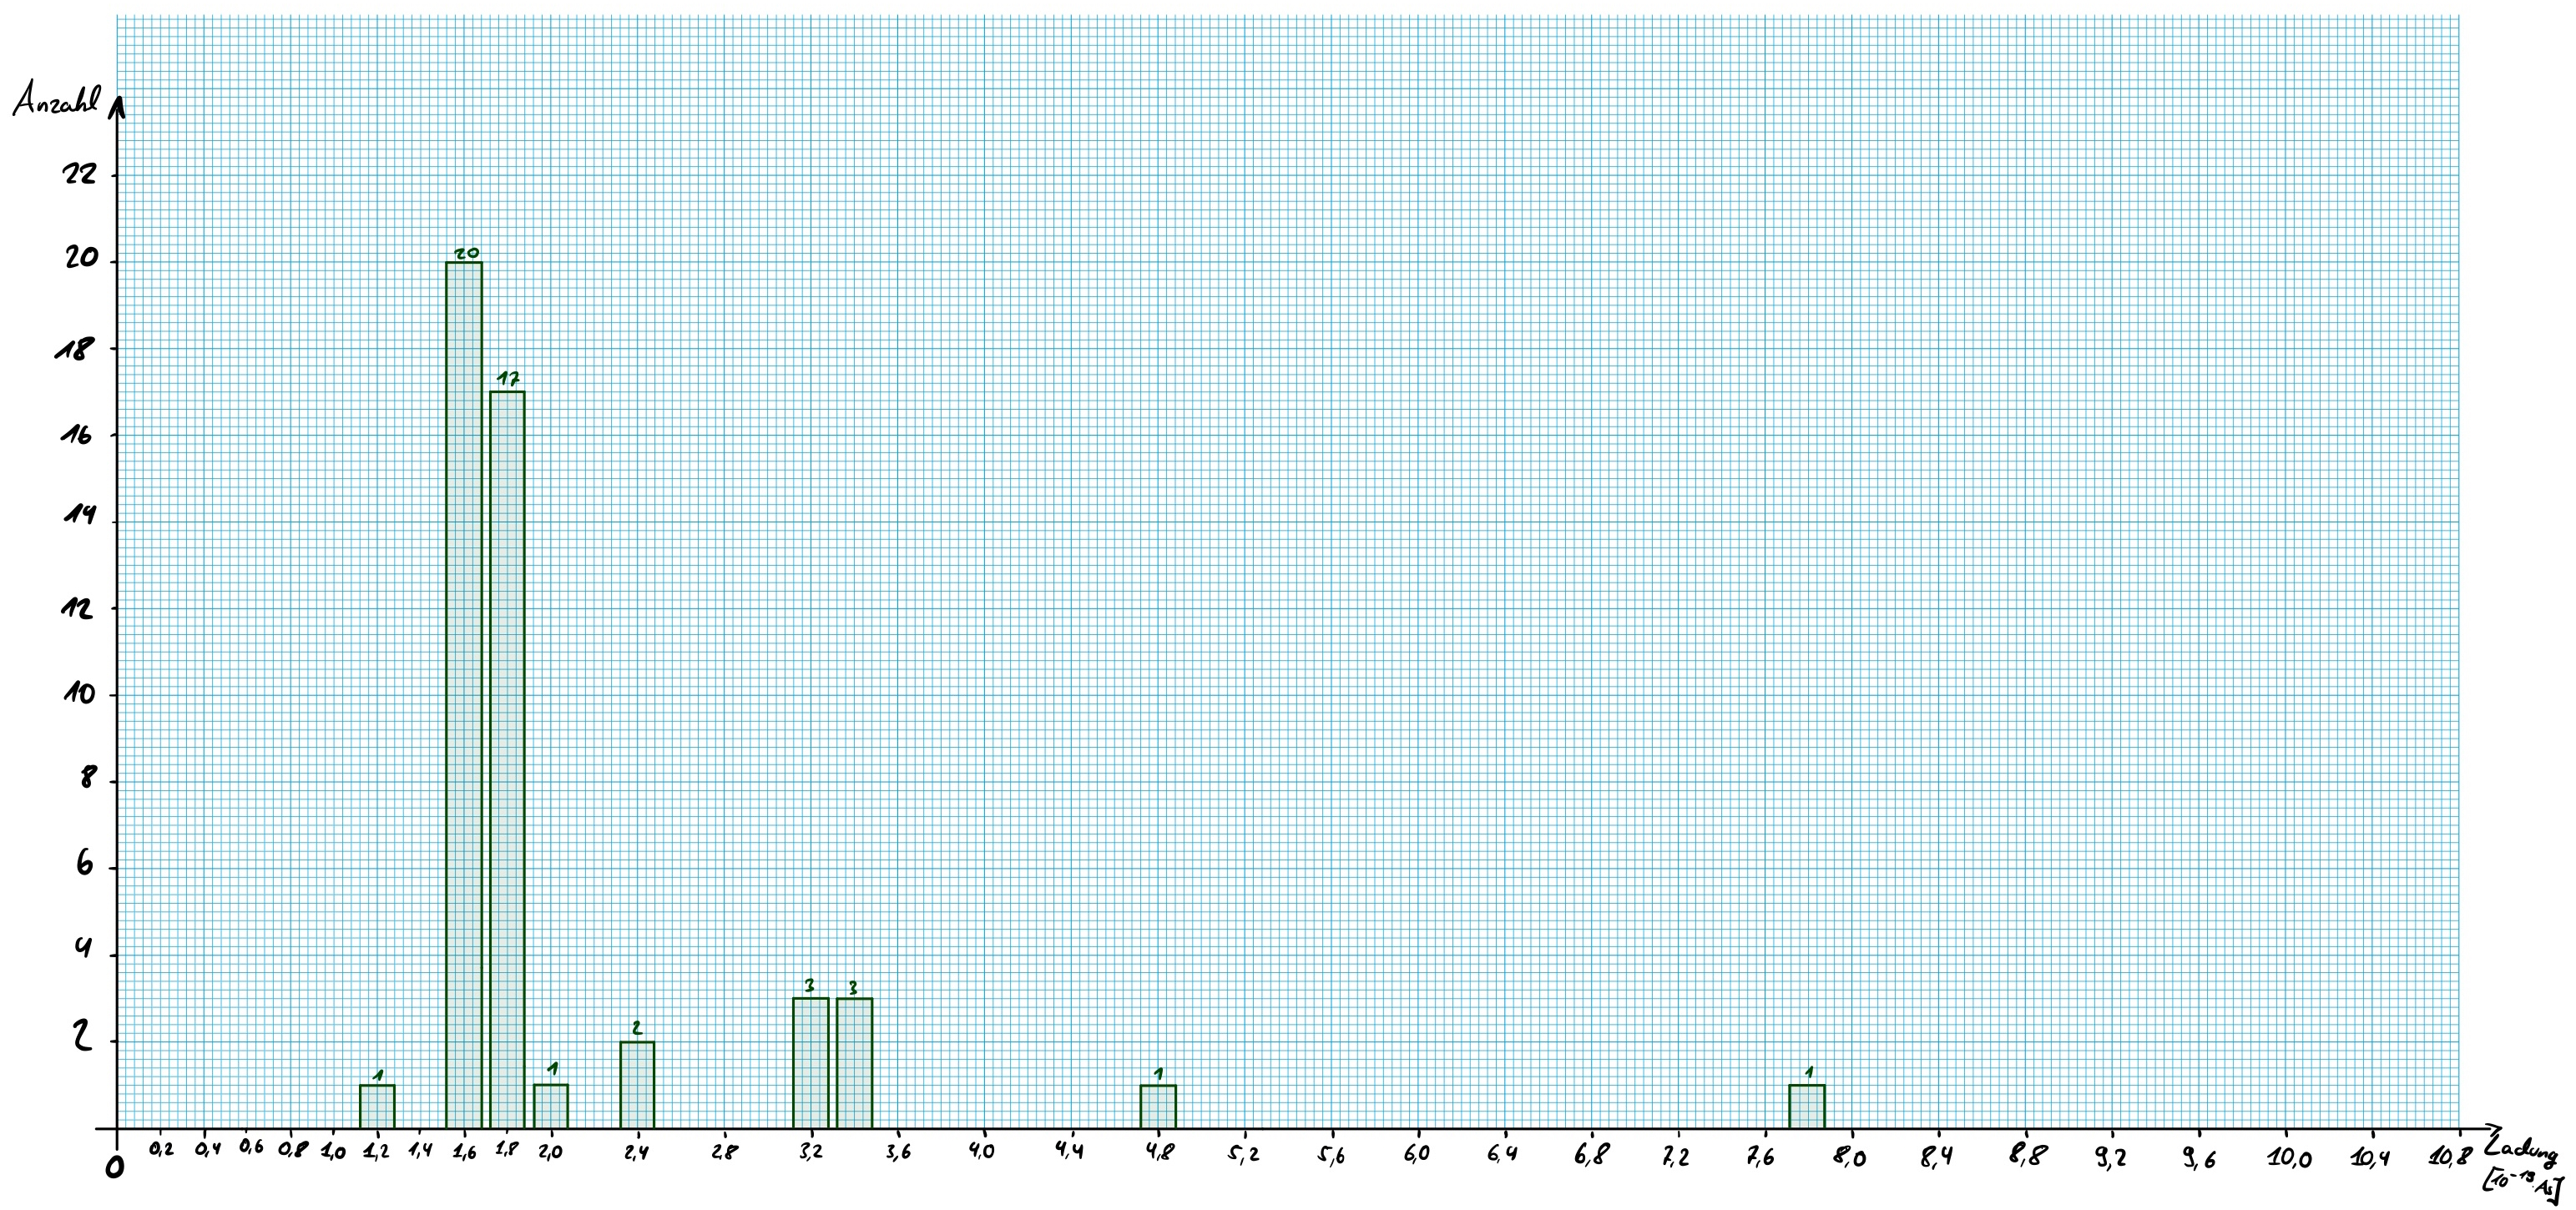
\includegraphics[height=0.6\textwidth, angle=90]{graphics/histoshit.jpg}
    \caption{Histogramm der gemessenen Ladungen}
    \label{fig:histoshit}
\end{figure}

\newpage

\subsection{Beurteilung der Excel-Werte}

Anhand des Histogramms kann man beurteilen, ob die von der Excel-Tabelle gewählte Begrenzung der Werte, die noch mit der Ladung $1e$ bezeichnet werden. In der Tabelle ist angegeben, dass der obere Grenzwert bei $2,4 \cdot 10^{-19}$As liegt. Dies entspricht im Vergleich mit dem Literaturwert $e_l = 1,602176634 \cdot 10^{-19}$As (Wikipedia, Stand 28.09.23) etwas weniger als 1,5$e_l$, was somit durchaus wie eine vernünftige Grenze wirkt. Allerdings gibt es zwei Werte, die direkt auf der Grenze bei 2,4 im Histogramm liegen, wovon einer von der Tabelle noch als eine Ladung gewertet wurde. Inwiefern sich dieser Wert negativ auf das Endergebnis auswirkt bleibt noch abzusehen, allgemein scheint die Grenze in Anbetracht der anderen Werte aber sinnvoll gewählt.

\subsection{Systematischer Fehler}

Zur Abschätzung der systematischen Fehler verwenden wir folgende Formel:

\begin{equation}
    \frac{\Delta q}{q} = \sqrt{\left( \frac{3\Delta s}{2s} \right)^2 + \left( \frac{\Delta \rho}{2 \rho} \right)^2 + \left( \frac{3 \Delta \eta}{2 \eta} \right)^2 + \left( \frac{\Delta d}{d} \right)^2 + \left( \frac{\Delta U}{U} \right)^2}
\end{equation}

Hierbei stammen die Vorfaktoren $\frac{3}{2}$ von den gleichwertigen Potenzen von $s$ und $\eta$ und die $\frac{1}{2}$ von der Potenz von $\rho$. Wir verwenden die folgenden Fehler:

\begin{equation}
    \begin{split}
        \Delta s &= 0,13 \cdot 10^{-5}\text{m} \\
        \Delta d &= 0,05 \text{mm} \\
        \Delta \rho &= 0,5\% \cdot \rho_{"o} = 4,36 \frac{\text{kg}}{\text{m}^3} \\
        \Delta U &= 0,5 \% \cdot U = 2,5 \text{V} \\
        \Delta \eta &= 2,0 \% \cdot \eta = 0,03 \cdot 10^{-5} \frac{\text{Ns}}{\text{m}^2} \\
    \end{split}
\end{equation}

Damit kommen wir auf folgenden relativen Fehler:

\begin{equation}
    \bm{\frac{\Delta q}{q}} = \bm{0,05}
\end{equation}

Wir kommen also auf einen systematischen Fehler von 5\%.

\newpage

\subsection{Statistischer Fehler}

Wir nehmen an, dass der statistische Fehler hauptsächlich vom Messfehler der Geschwindigkeitsmessungen abhängt und schätzen diesen mit unseren Messwerten aus Tabelle 1 ab. Dazu berechnen wir die Ladungen mit den gemachten Messungen und bestimmen den Fehler einer Einzelmessung $\sigma_q$.


\begin{table} [!h]
    \centering
    \caption{Bestimmung der Ladung \& Fehler der Einzelmessung}
    \resizebox{\textwidth}{!}{
    \begin{tabular}{c|c|c|c|c|c|c|c}
        \hline
        $\bm{t_{f}}$ [s] & $\bm{t_{s}}$ [s] & $\bm{v_{f}}$ [m/s] & $\bm{v_{s}}$ [m/s] & $\bm{r_0}$ [m] & $\bm{f(r_0)}$ & $\bm{q}$ [As] & $\bm{\sigma_q}$ [As] \\ \hline
        23,55 & 10,87 & $4,46 \cdot 10^{-5}$ & $9,66 \cdot 10^{-5}$ & $6,52 \cdot 10^{-7}$ & 0,8943 & $3,189 \cdot 10^{-19}$ & \\
        21,19 & 10,31 & $4,96 \cdot 10^{-5}$ & $10,18 \cdot 10^{-5}$ & $6,88 \cdot 10^{-7}$ & 0,8992 & $3,634 \cdot 10^{-19}$ & \\
        22,52 & 10,91 & $4,66 \cdot 10^{-5}$ & $9,62 \cdot 10^{-5}$ & $6,67 \cdot 10^{-7}$ & 0,8964 & $3,312 \cdot 10^{-19}$ & $0,166 \cdot 10^{-19}$\\
        22,09 & 11,06 & $4,75 \cdot 10^{-5}$ & $9,49 \cdot 10^{-5}$ & $6,74 \cdot 10^{-7}$ & 0,8973 & $3,340 \cdot 10^{-19}$ & \\
        22,45 & 10,98 & $4,68 \cdot 10^{-5}$ & $9,56 \cdot 10^{-5}$ & $6,68 \cdot 10^{-7}$ & 0,8965 & $3,307 \cdot 10^{-19}$ & \\ \hline
    \end{tabular} }
    \label{tab:fehler}
\end{table}

Nun kann man noch mit der Anzahl der gemittelten Werte $n=5$ den Fehler des Mittelwerts $\Delta \overline{q}$ berechnen:

\begin{equation}
    \begin{split}
        \Delta \overline{q} &= \frac{\sigma_q}{\sqrt{n}} \\ \\
        \bm{\Delta \overline{q}} &= \bm{0,07 \cdot 10^{-19}} \textbf{As}
    \end{split}
\end{equation}

In der Excel Tabelle wurde als Standardabweichung einer Einzelmessung $0,191 \cdot 10^{-19}$ angegeben. Wie man erkennen kann, ist der Wert aus Tabelle \ref{tab:fehler} etwas kleiner. Dies mag daran liegen, dass bei den fünf Messungen genau das gleiche Teilchen fünf mal gemessen wurde, während die Werte in Excel von vielen verschiedenen Teilchen stammen. Jedoch ist beim Fehler des Mittelwerts der Excel-Wert mit $0,027 \cdot 10^{-19}$ viel genauer als unser Wert, da in der Excel Tabelle nicht nur fünf, sonder fünfzig Werte gemittelt wurden.

\newpage

\subsection{Vergleich mit dem Literaturwert}

Zum Abschluss vergleichen wir den von Excel bestimmten Mittelwert sowie Fehler des Mittelwerts mit dem Literaturwert. Dazu addieren wir zunächst den von statistischen Fehler des Mittelwerts mit unserem systematischen Fehler, den wir aus dem relativen Fehler mit dem Mittelwert bestimmen, quadratisch, um den endgültigen Ladungsfehler $\Delta e$ zu erhalten: 

\begin{equation}
    \begin{split}
        \Delta q_{sys} &= e \cdot \left( \frac{\Delta q}{q} \right) =  0,08 \cdot 10^{-19} \text{As} \\
        \Delta e &= \sqrt{(\Delta q_{sys})^2 + (\Delta \overline{q})^2} = 0,11 \cdot 10^{-19} \text{As}
    \end{split}
\end{equation}


Somit kommen wir auf folgendes Endergebnis:

\begin{equation}
    \bm{e} = \bm{(1,653 \pm 0,11) \cdot 10^{-19}} \textbf{As}
\end{equation}

Der Vergleich läuft über einen Signifikanztest:

\begin{equation}
    \begin{split}
        \sigma = \frac{|e-e_{Lit}|}{\Delta e} = 0,46
    \end{split}
\end{equation}
%\sqrt{(\Delta e)^2} + (\Delta e_{Lit})^2
Diese Abweichung ist innerhalb des $3\sigma$-Intervalls und somit nicht signifikant.

\newpage
%---------------PRÄSENTATION DER ENDERGEBNISSE---------------
\section{Präsentation der Endergebnisse}

In diesem Versuch wurde die Elementarladung bestimmt als 

\begin{equation}
    \bm{e} = \bm{(1,653 \pm 0,11) \cdot 10^{-19}} \textbf{As}.
\end{equation}

Dieses Ergebnis hat eine Sigmaabweichung von $\sigma = 0,46$ zum Literaturwert.

\newpage
%---------------ZUSAMMENFASSUNG UND DISKUSSION---------------
\section{Zusammenfassung und Diskussion}

In diesem Versuch wurde mithilfe des von Millikan veröffentlichen Verfahrens die Elementarladung bestimmt. Wir betrachteten fünfzig Öltröpfchen im Plattenkondensator und bestimmten deren Fall- sowie Steiggeschwindigkeiten, um in Endeffekt daraus deren Ladung zu bestimmen. Durch die Fokussierung auf langsam fallende und steigende Tröpfchen konnten so vorüberwiegend Teilchen mit einer Elementarladung untersucht werden.

Zunächst lässt sich zum Ergebnis positiv vermerken, dass es mit einer Abweichung von $\sigma = 0,46$ sehr nah am Literaturwert liegt, dies trotz dem prozentual recht kleinen Fehler von 6,65\%. Da die Auswertung praktisch komplett über die gestellte Excel-Tabelle lief und sich unsere manuelle Auswertung nur auf die Überprüfung eines zufälligen Wertes, die Beurteilung der Abschätzungen der Tabelle sowie die Berechnung der Fehler beschränkte, lassen sich hier auch keine wirklichen potenziellen Fehlerquellen in der Auswertung selbst finden. Dafür gibt es noch ein paar nennenswerte Punkte zur Versuchsdurchführung.

Zunächst lässt sich vermerken, dass die Messung der Zeit, die ein Tröpfchen beim Steigen oder Fallen brauchte, komplizierter war, als es schien. Häufig waren die ausgewählten Tröpfchen durch die teilweise unzureichende Auflösung des Bildes auf dem Bildschirm nach halber Strecke nicht mehr erkennbar oder verschwammen mit anderen Tröpfchen und das trotz vorheriger Scharfstellung des Bildes. Auch war es schwierig abzuschätzen, welche Strecke man überprüfen sollte, da sich die horizontalen Linien auf dem Bildschirm bis auf den Nullwert praktisch nicht mit Markierungen der Skala überschnitten.

Verbesserungen bei der Durchführung hätten erzielt werden können, indem man beispielsweise längere Strecken nimmt um die Zeit zu messen, da so der Zeitfehler minimiert werden würde, oder eine stärkere Vergrößerung der Tröpfchen mit einem stärkeren Mikroskop erzielt. 

Zusammenfassend lässt sich sagen, dass trotz der genannten potenziellen Fehlerquellen ein gutes Ergebnis erzielt werden konnte, das nicht signifikant vom Literaturwert abweicht. Somit wird sehr gut klar, wie beeindruckend gut der von Millikan eingeführte Versuch sogar im Rahmen dieses Praktikums funktioniert, was seine Relevanz in der Physik und die Verleihung des Nobelpreises begründet. 

\end{document}

